% document layout
\documentclass[12pt]{report}
\usepackage[utf8]{inputenc}
\usepackage{graphicx}
\usepackage[export]{adjustbox}
\usepackage{amsmath,mathtools}
\usepackage[subpreambles=true]{standalone}
\usepackage[document]{ragged2e}
\usepackage[english]{babel}
\usepackage{siunitx}
\usepackage{cite}
\usepackage{braket}
\usepackage{geometry}
\geometry{left = 2cm,right = 2cm,top = 4cm}


% packages
\usepackage{graphicx}
\graphicspath{ {images/} }
\usepackage{float}
\usepackage{gensymb}
\usepackage{datetime}
\usepackage{appendix}
\usepackage{amsmath}
\usepackage[stable]{footmisc} %for footnote in title
\usepackage{fancyhdr}
\usepackage{caption}
\usepackage{listings}
\lstset{captionpos=b} % set the caption position to bottom

\title{

\includegraphics[width=0.25\textwidth]{nus_logo.jpeg}
\includegraphics[width=0.32\textwidth]{cqt_logo.png}\\
{\LARGE \textbf{Laser Frequency Stabilisation for The Ion Trap Quantum Processor}}\\
\vspace{5mm}
{\normalsize A report submitted in partial fulfillment for the courses}\\
{\normalsize PC3288 - \textit{Advanced UROPS in Physics I}}\\
{\normalsize PC3289 - \textit{Advanced UROPS in Physics II}}
}

\author{
{\normalsize Lin Zhonglin \hspace{10mm} A0222183N}\\
\vspace{1mm}
{\normalsize Supervisor: Professor Dzmitry Matsukevich}\\
{\normalsize Assessor: Professor Dzmitry Matsukevich}\\
{\normalsize Assessor: Doctor Jaren Gan }}\\
\date{{\normalsize Department of Physics}\\
{\normalsize National University of Singapore}\\
{\normalsize Apr 2023}}

\linespread{1.2}
\setlength{\parskip}{1em}
\setlength{\parindent}{0pt}

\begin{document}
\maketitle

\chapter*{Abstract}
As lasers are used to address atomic energy level transitions in atomic and molecular physics laboratory, it is of great importance to generate high quality lasers beams. This report first discusses the repair and tuning of a compact grating-stabilized External Cavity Diode Laser system (ECDL). Secondly, this report discusses the process of locking a cavity to a master laser through a standard Pound-Drever-Hall (PDH) scheme and possible uses of such a locked cavity. 


\chapter*{Acknowledgements}
I would like to thank Associate Professor Dzmitry Matsukevich for this opportunity to gain in- valuable experience in a research laboratory.
I would also like to thank my colleagues and seniors who I have spent time with over the year in Dzmitry Labs: Jaren, Mu Young, Ko Wei, Rongjie, Nigel, Ka Hui and Dillon. I would especially like to thank my project mentors, Jaren and Mu Young, for all their help and advice given throughout the project. I would also like to thank all the professors and seniors in CQT that gave me a helping hand during my research struggle. 
I would also like to thank my parents for being very supportive of me.
This project would not have been possible without the superb people mentioned.

\tableofcontents

\chapter{Introduction}
In the ion trapping laboratory of professor Dzmitry Matsukevich, Ytterbium 171 ions are trapped for state manipulation and detection. Some main energy levels under interest of Ytterbium 171 ions are shown in Fig \ref{fig:Yitterbium171Ion}. Energy level transition between  $^2 S_{1/2}$ F=0 and $^2 S_{1/2}$ F=1 is the main energy level of interest, a 369.5261nm laser beam is used to address the energy level transition between the two states through Raman transition. When the trapped ion is in any of these two states, it fluoresces and can be captured by a photodetector. There exists some probabilities that the trapped ion might transit to the energy states displayed towards the right of Fig \ref{fig:Yitterbium171Ion}. To optically pumped the ion out of these "dark states", 935.1879nm and two $\approx$ 638nm laser beams are used. Original a compact grating-stabilized External Cavity Diode Laser system of frequency $\approx$ 638nm was used to generate the $\approx$ 638nm laser beam but suffered a diode failure. I replaced the diode and tuned the laser back to the needed frequency. In this report I document the procedure and relevant information. 
\\
\par
As the transition to the $^2 D_{3/2}$ states is quite probable, the 935.1879nm laser has to be kept on most of the time to continuously pump the trapped ion back to bright states. Hence, effort is needed to frequency lock the laser. One way to achieve this is to lock the laser to a cavity which is locked to a master laser (assumed frequency stable) through a standard Pound–Drever–Hall (PDH) technique. 

\begin{figure}[H]
    \centering
    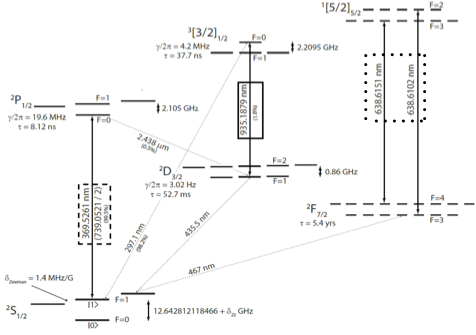
\includegraphics[width=\textwidth]{Yitterbium171Ion.png}
    \caption{Partial level structure for Ytterbium 171 ion \cite{DemonstrationOfRabi-FlopsWithYtterbium171Trapped-IonQubits}
    }
    \label{fig:Yitterbium171Ion}
\end{figure}


\chapter{Building And Tuning A Compact 638nm Grating Stabilized Diode Laser System}/
\section{Theory and Laser Frequency Tuning}
Since their first use in atomic physics in the early 80's, diode lasers have become an important part of many modern experiments. This is primarily due to the high reliability and the low price of these devices which facilitate experiments involving a number of lasers operating at different frequencies \cite{compactGratingDiodeLaser}.
\par
This section of the report discusses a compact grating-stabilized External Cavity Diode Laser (ECDL) system. Here, I focused on fixing an existing 638nm laser system that had suffered from a diode failure. I replaced the diode (Thorlabs, L638P040 - 638 nm, 40 mW, Ø5.6 mm pin diode) and tuned the laser around 638.61nm of wavelength for optically pumping Ytterbium ion out of the ${ }^2 F_{7 / 2}$ hyperfine states (See red-boxed transition in Fig \ref{fig:Yitterbium171Ion}. Laser light of wavelengths of 638.6102nm and 638.6151nm are used to drive the transitions ${ }^2 F_{7 / 2}|F=3\rangle \leftrightarrow{ }^1[5 / 2]_{5 / 2}|F=2\rangle \text { and }{ }^2 F_{7 / 2}|F=4\rangle \leftrightarrow{ }^1[5 / 2]_{5 / 2}|F=3\rangle$ respectively. (See Fig \ref{fig:Yitterbium171Ion}) As the transition of the trapped ion to these states are no very probable, is neither fine tuned nor frequency locked. Jumping between the two transitions is done by manually tuning the injection current(details on frequency tuning will be discussed later). The main sources for this section of the report are \cite{compactGratingDiodeLaser}\cite{fundamentalsOfPhotonics}.

\begin{figure}[H]
    \centering
    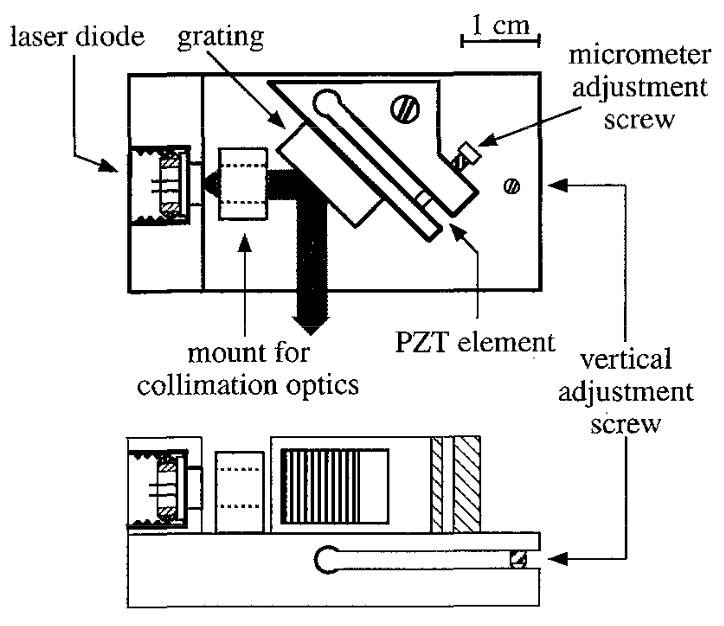
\includegraphics[width=.8\textwidth]{compactDiodeLaserSchematics.png}
    \caption{Schematics of the mechanical setup of the grating-stabilized diode laser system. \cite{compactGratingDiodeLaser}
    }
    \label{fig:compactDiodeLaserSchematics}
\end{figure}

\begin{figure}[H]
    \centering
    \includegraphics[width=.8\textwidth]{638laserSetup.png}
    \caption{638nm Laser Actual Setup}
    \label{fig:638laserSetup}
\end{figure}

A free-running diode suffers from having a large linewidth. In the context of ion trapping laboratory, large linewidth can result in reduced cooling efficiency, unintended energy level transitions or undesired coupling to nearby energy level and so on. An optical cavity that provides optical feedback can greatly reduce the output linewidth. How an external cavity affects emission wavelength will be discussed later. In the system under discussion, the first-order diffracted light from the diffraction grating is coupled back into the diode, so that the grating and the diode form an external resonator. The use of a diffraction grating in the current setup results in a linewidth reduction of two orders of magnitude and it also allows for the selection of any desired wavelength as the external cavity length can be adjusted\cite{compactGratingDiodeLaser}.The external cavity length (distance between grating and facade of diode) is chosen to be about 15mm optimise for single mode operation according to \cite{compactGratingDiodeLaser}. A peltier element is embedded in the mechanical structure to maintain temperature of the system. A piezo actuator is placed behind the grating to allow small adjustments and scanning of the external cavity length and angle. (See \cite{compactGratingDiodeLaser} for more details)
\par
To tune the emission wavelength of an ECOL, consider the following picture. The gain profile of a typical laser diode has a width of 10nm \cite{compactGratingDiodeLaser}. The emission wavelength is determined by the competition between the longitudinal modes of the laser cavity, which are typically separated by 100-200 GHz\cite{compactGratingDiodeLaser}. The laser operates at the mode which experiences the maximum gain (See Fig \ref{fig:diodeLaserGainCurve}. In this picture, the maximum gain happens at where the four main gain profiles overlapped the most. In Fig \ref{fig:diodeLaserGainCurve}, mission frequency is likely to be in the red marked region. 
\begin{figure}[H]
    \centering
    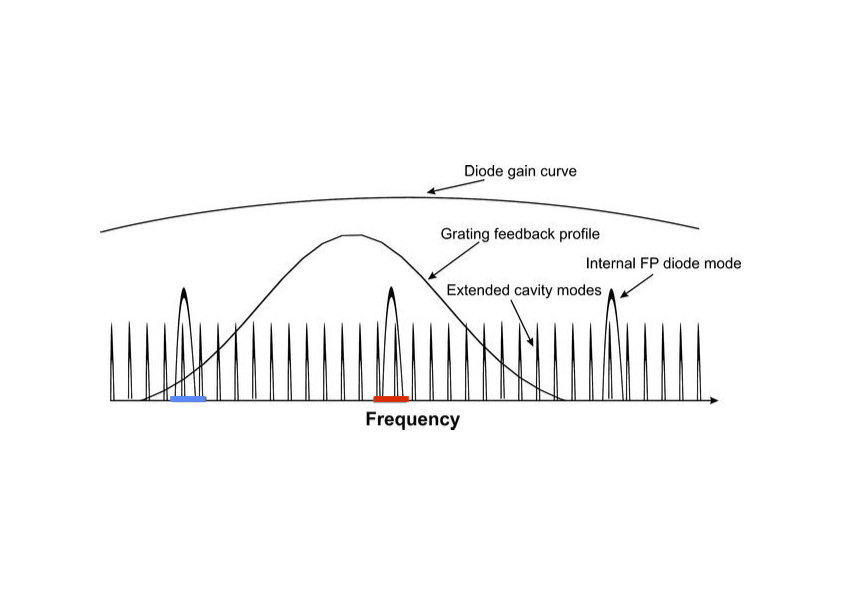
\includegraphics[width=.8\textwidth]{diodeLaserGainCurve.png}
    \caption{Schematic representation of mode competition in an ECDL\cite{DiodeLaserInducedFluorescenceForGas-PhaseDiagnostics}}
    \label{fig:diodeLaserGainCurve}
\end{figure}
There are three fine-tunable parameters that affect the emission wavelength: the temperature, piezo voltage and the injection current (to the diode): 
\begin{enumerate}
    \item Temperature variations cause a change of the cavity length (and thus a change of the resonance frequencies of the longitudinal modes) and at the same time a frequency shift of the gain profile. Consequently, the emission wavelength can be tuned with the temperature. However, in the process of tuning, the gain of the modes varies such that at some point the laser emission frequency jumps from one mode to another (commonly referred to as \textbf{mod-hopping}), resulting in a number of inaccessible frequency domains. For instance in Fig \ref{fig:diodeLaserGainCurve}, if the Grating feedback profile is continuously shifted to the left emission frequency might jump from the red-marked region to the blue-marked region as the region of maximum overlap changes. \cite{compactGratingDiodeLaser} suggests that the width of the accessible frequency domain is typically a fraction of the spectral range of the laser cavity. Here with laser cavity being 15mm, it's several tens of GHz.

    \item A second parameter that can be used to tune the emission wavelength is to vary the injection current. This leads to a corresponding temperature change and also a change of the carrier density and thus of refractive index of the semiconductor material. Injection current tuning also suffers from mode hopping. However, as we want to tune the wavelengths of the laser bewteen 638.6102nm and 638.6151nm to address two different state transitions quickly, we need a modhopping-free region that at least covers these two wavelengths. The solution is to vary the injection current and the piezo voltage synchronously so as to lower the probability of mod hop. As shown in Fig \ref{fig:638Driver}, from left to right are accordingly the laser driver, coefficient gain board and the piezo voltage supply. As the piezo votlage is varied, it supplies a sync output to the coefficient gain board which then outputs a proportional volage to the laser driver whcih offests the injection current such that the gain curve of injection current and grating move synchronously. 
\end{enumerate}

\begin{figure}[H]
    \centering
    \includegraphics[width=.8\textwidth]{638Driver.png}
    \caption{638nm laser driver boards}
    \label{fig:638Driver}
\end{figure}
 
After careful replacement of the original dead diode, coarse adjustment of the wavelength is achieved by horizontally tilting the grating with the micrometer screw. The main goal now is to vary the temperature and injection current in search for a mode-hopping-free region in the gain profile near the desired wavelength of around 638.615nm. Fig \ref{fig:diodeLaserEW} shows a few tens of data points of temperature-EW plots. The bottom data points from a dense grid as expected, showing that it's a mode-hop-free region. Whereas the top few data points probably is a result of mode hopping. After many trial and error, the final set of parameters arriving at EW=638.615nm is [set temperature for the peltier = 17.92$\degree$, set current = 52.3mA, current offset = -0.563 mA, piezo voltage = 2.5 V However, this EW still suffers from drifting. 
%TODO: explain the current offset here

\begin{figure}[H]
    \centering
    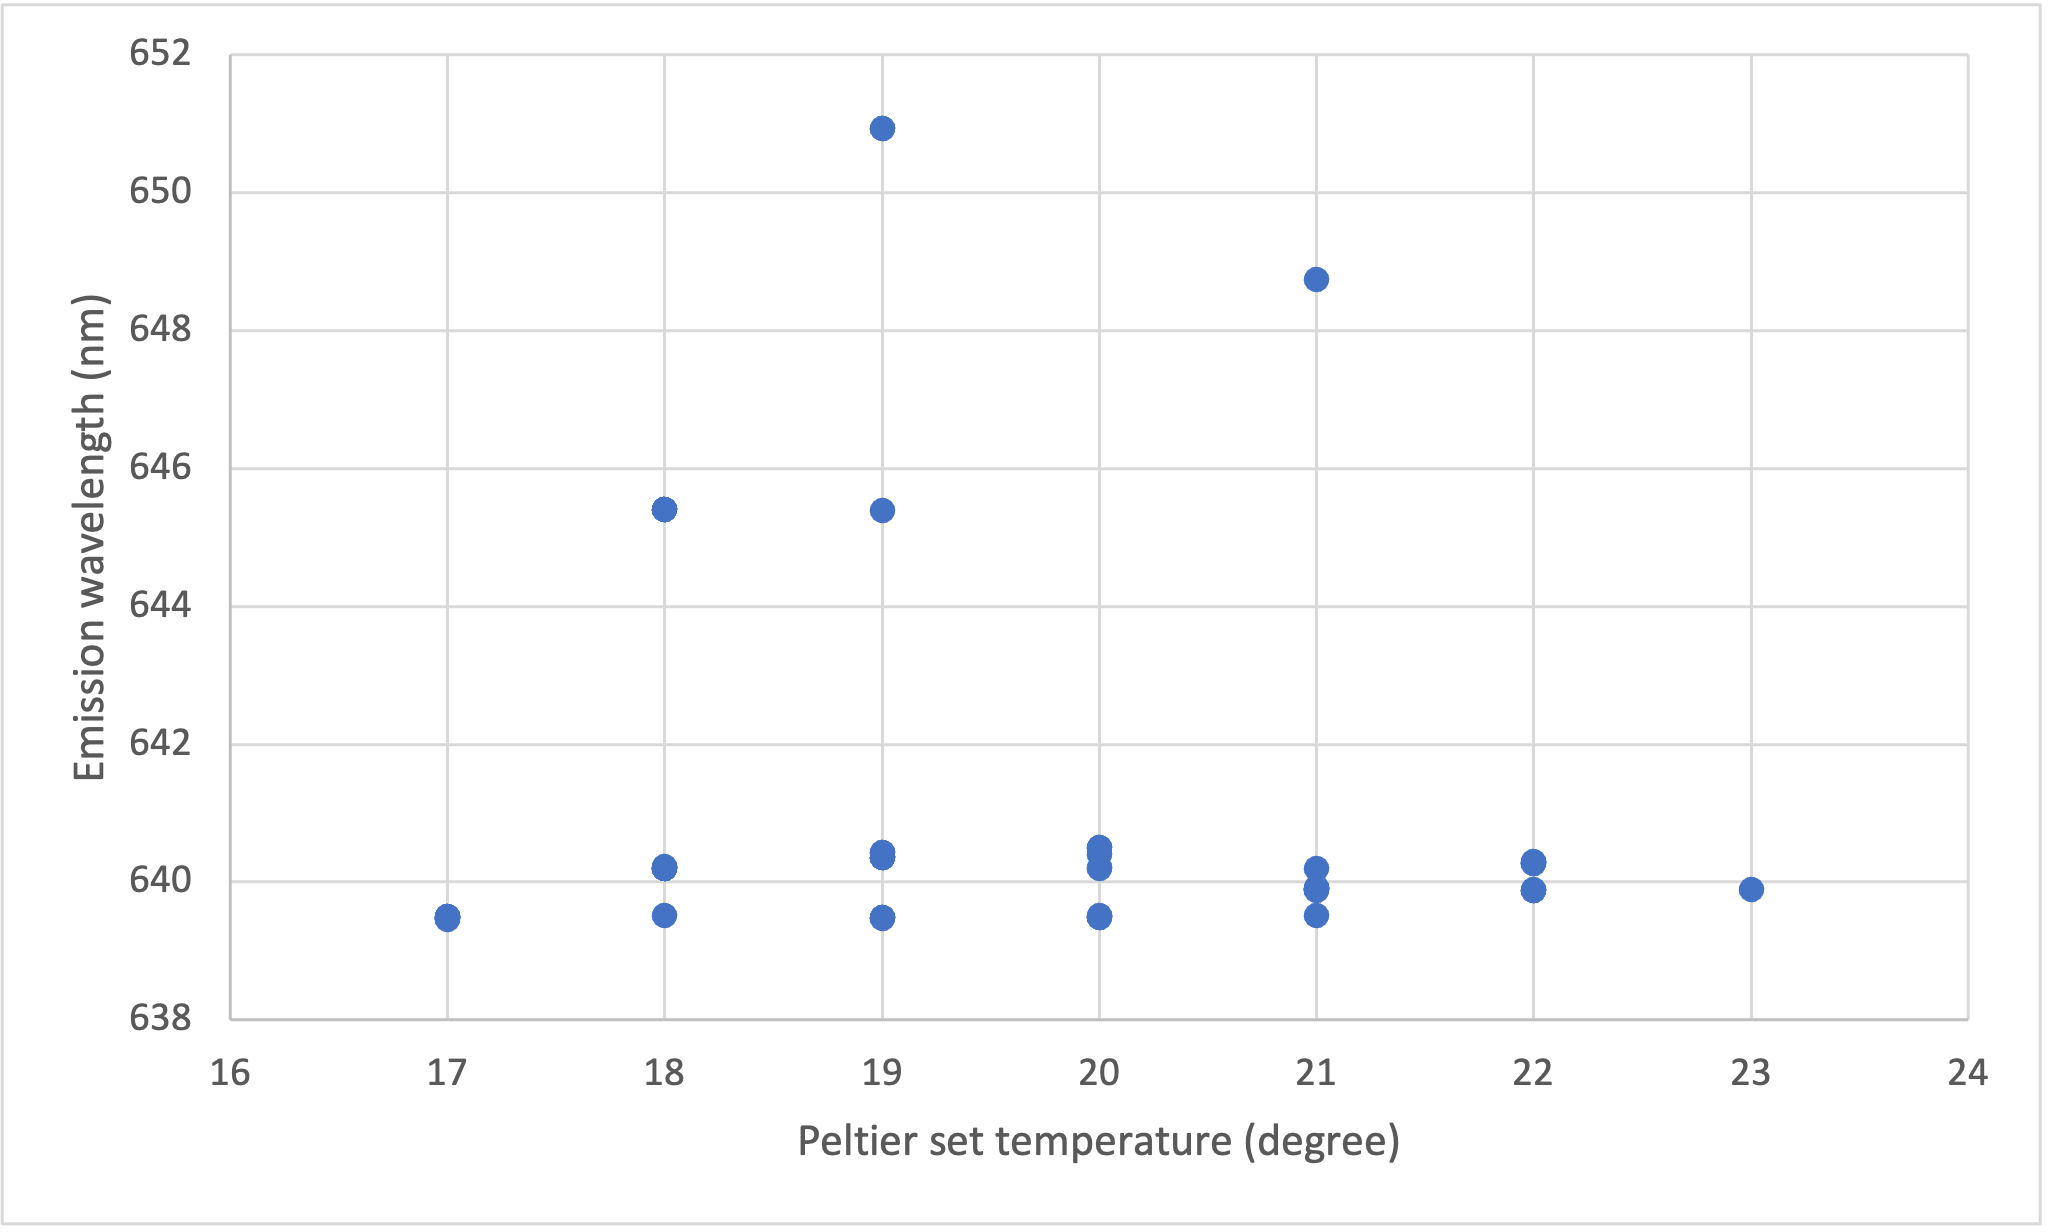
\includegraphics{diodeLaserEW.png}
    \caption{Diode EW - temperature}
    \label{fig:diodeLaserEW}
\end{figure}

\section{Gaussian Beam Characterisation and collimation}
%TODO: add some gaussian beam theory here
When dealing with laser beams, Gaussian beam optics is commonly considered. As the laser diode has a rectangular shape, its initial output laser beam has an oval shape and thus not very Gaussian and not very suitable for subsequent Gaussian beam characterisation and coupling to optical fibres. A pair of anamorphic prism is first used to tune the laser beam cross section to be as circular as possible. (See the two red-glowing prisms in Fig \ref{fig:638laserSetup}) Next, it's desirable to collimate the beam for ease of coupling into other optical components. Coarse collimation can be done by eyeballing the change of the beam spot diameter at different distance from the collimating lens and adjusting the position of the collimating lens to make beam spot diameter as constant as possible across the scanning distance. To achieve finer collimation, consider the following Gaussian beam characterisation process: 
\par
First we need to measure the beam spot diameter at different distances from the collimating lens. To do so, consider the knife edge measurement for very precise measurement. Alternatively consider using a CCD camera for measurement for precision of up to $\mu m$ level precision (size of CCD pixels). 
\par
To do a proper knife edge measurement, refer to \cite{KnifeEdgeMeasurement} for details. A piece of paper blade is painted with black paint to use as the blocking knife edge. Black paint is to reduce reflection of laser beam. The black-painted paper blade is then mounted onto a translational stage as shown in Fig \ref{fig:knifeEdgeMeasurementSetup}. Position the blade perpendicular to the laser beam. Place a photodiode behind the blade as shown in Fig \ref{fig:knifeEdgeMeasurement} and connect the photodiode to an Arduino. Finally connect the Arduino to a computer and run code \ref{code:knifeEdgeMeasurementDataCollection} in Annex. The code collects three sets of voltage reading from the photodiode and take average. Move the knife edge to block more light by rotating the translational stage. run code \ref{code:knifeEdgeMeasurementDataCollection} in Annex again. Repeat the previous steps until reading from the photodiode is close to background reading. Now input the distance (of knife edge) - photodiode voltage data from previous steps to code \ref{code:knifeEdgeMeasurementDataProcessing} in Annex for data processing. This code fits the distance-voltage data to an error function and outputs a fitted value of the laser beam width. 

\begin{figure}[H]
    \centering
    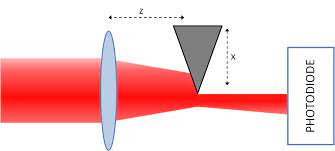
\includegraphics[width=.6\textwidth]{knifeEdgeMeasurement.jpeg}
    \caption{Knife Edge Measurement}
    \label{fig:knifeEdgeMeasurement}
\end{figure}

\begin{figure}[H]
    \centering
    \includegraphics[width=.8\textwidth]{knifeEdgeMeasurementSetup.png}
    \caption{Knife edge measurement estup}
    \label{fig:knifeEdgeMeasurementSetup}
\end{figure}

Although the aforementioned knife edge measurement with a knife blade is can be very precise up to the limit of diffraction caused by the blade, it's very time consuming without the translational stage being automated. With time constraint, a less precise (up to $\mu m$ level) yet much faster method with a CCD camera can be employed. Place a camera such that the laser beam spot falls completely on the CCD sensor. Run code \ref{gaussianBeamCharacterisation} in Annex to measure the laser beam spot horizontal and vertical radius at the position of the CCD sensor. The find horizontal radius, the code sums up all rows of pixels and filter for pixels exceeding $1/e^2$ of the pixel with maximum reading. Then take the right most pixel position minus the left more pixel position as an estimate of the beam spot diameter. The code runs similarly for vertical beam spot radius. For details, see code \ref{code:gaussianBeamCharacterisation} in Annex. I used a Point Grey Research Chameleon CMLN-13S2M CCD camera with pixel size 3.75 µm for data taking. Pixel size is important here as it determines the error margin of my final estimated beam diameter. To use \ref{code:gaussianBeamCharacterisation} as it is, take a background image and 5 beam images at differnt z-positions. Name the files according to README and run the script to get an estimation of the horizontal and vertical beam radius. Adjust the collimating lens accordingly to make the beam waist z position as far as possible. 
\\
\par
In order to monitor the laser system emission wavelength, part of the laser beam power is sent to the wavemeter via a fiber. To send a laser beam into a single-mode optical fibre is to couple their spatial modes, follow the procedure listed in Appendix \ref{appendix:laerFibreCoupling}. In red rectangle of Fig \ref{fig:638laserSetup}, the left fibre mount is used to send partial laser power to the wavemeter for wavelength monitoring and the right fibre mount is used to send laser beam to the ion trap for use. 

\chapter{Locking A F-P Cavity To A Master laser Through PDH Technique}
Tunable lasers have multiple wavelength-selecting elements such as piezo-controlled etalons and gratings. Typically, the length of the lasing cavity is controlled by a voltage sent to a piezo-electric transducer. The laser-cavity length can change because of a number of factors such as temperature changes, and mechanical vibrations. These factors affect the laser-frequency stability. The standard PDH method of frequency-locking involves the following process: A laser's frequency is measured with a Fabry-Perot cavity, and this measurement is fed back to the laser to suppress frequency drift\cite{PDH1983}\cite{PDHintro}.
\par
\begin{figure}[H]
    \centering
    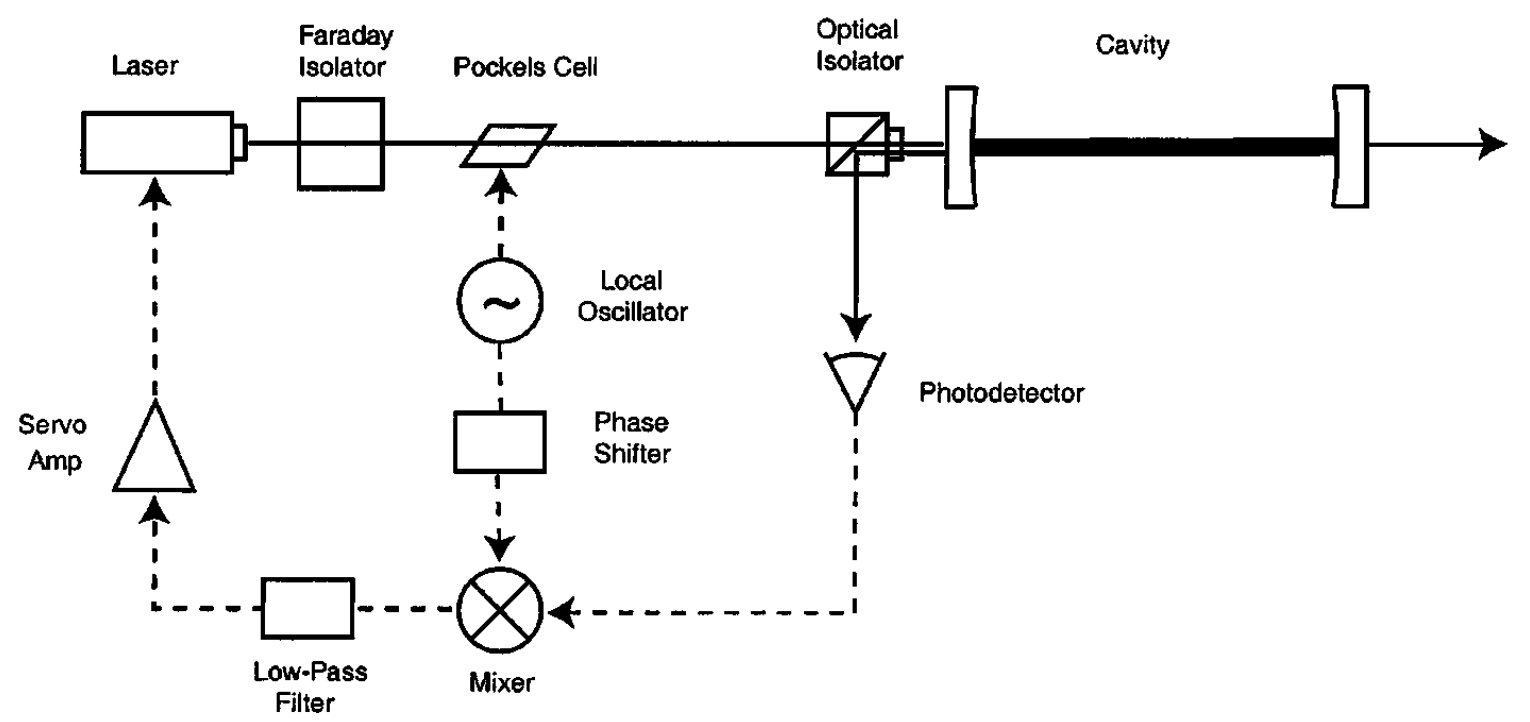
\includegraphics[width=.8\textwidth]{PDHlayout.png}
    \caption{The basic layout for locking a cavity to a laser. Solid lines are optical paths and dashed lines are signal paths. The signal going to the laser controls its frequency \cite{PDHintro}}
    \label{fig:PDHlayout}
\end{figure}

Referring to Fig \ref{fig:PDHlayout}, the basic steps of a PDH locking scheme are outlined as following: 
\begin{enumerate}
    \item A laser beam is passed through a Pockels cell to modulate its frequency at a frequency small relative to the $\Delta \nu_{fsr}$ free spectral range of the optical cavity. My cavity has length $L=15$cm, $\Delta \nu_{fsr} = c/2L \approx 1GHz$. Hence my EOM at $\approx 38 MHz$, as discussed in the EOM section, is appropriate here. Note that EOM only modulates light of polarisation parrallel to the EOM's oscillating electric field. In my case horizontal polarisation w.r.t the optical table is used. (i.e. a quarter-wave-plate and half-wave-plate pair is used to clean up laser beam polarisation to be horizontal before entering the EOM) 

    \item The beam goes do the cavity. An optical isolator is used to pick up reflected beam from the cavity. I used a quarter wave plate and a polarising beam splitter. 

    \item Referring to Fig \ref{fig:cavityTransmission}, if length of the cavity is set to one side of these resonances, but near enough that some light gets transmitted, then a small change in laser frequency would produce a proportional change in the transmitted intensity. Equivalently there will be a change in the reflected beam intensity. Optimising for minimum reflection has the following benefits over optimising for maximum transmission: 
    \begin{enumerate}
        \item Effect of laser frequency drift and intensity drift is decoupled due to obvious reason.
        \item The frequency of frequency drift that can be corrected for is not restricted by the cavity response time. As when measuring transmission intensity, it takes time for the fields in the cavity to re-equilibrate whenever there is frequency drift. Whereas measuring reflected intensity circumvents this issue. 
    \end{enumerate}

    \item In order to have a control loop that locks the laser to a certain frequency, we need an error signal that tells provides a $\pm$ sign for the feedback signal on top of the amplitude as given by the last point. To obtain an error signal, the EOM comes into play in that it varies the laser frequency slightly (small w.r.t cavity free spectral range as discussed earlier), indicating whether laser frequency is currently on the right side or left side of resonance. 

    \item What's left is to produce an error signal by using a fast photodiode (fast enough to discern MHz level modulation) to read beam intensity coming from the optical isolator. Signal from the fast photodiode is then processed as shown in Fig \ref{fig:PDHlayout}. For details on how the multiplicative mixer and the phase shifter helps output an error signal, see \cite{PDHintro}.

    \item Caution: Note that wave plates and polarising beam splitter are wavelength rated
\end{enumerate}

%TODO: insert image of my setup here
%TODo: insert image of error signal here
\section{EOM (Electro-optic Modulator)}
% put basic intro to an EOM here 
In certain types of crystals it is possible to effect a change in the index of refraction that is proportional to the applied electric field. This is known as the Pockels effect. Applying a modulated electric field across such a crystal (usually the KDP type) and passing a beam of laser through the crystal leads to the laser beam being modulated in phase. (detail see: \cite{fundamentalsOfPhotonics}) 

\subsection{Theory and Model}
When a time-varying electric field is applied to the nonlinear crystal inside the EOM, the index of refraction $n$ changes in a sinusoidal manner resulting in phase modulation of the laser beam passing through the crystal. Consider the following short mathematical example to see that phase modulation is equivalent to frequency modulation: 
\\
% 见激光原理for this part
Suppose instantaneous electric field at a point of EM wave of a laser beam: 
\begin{align*}
    E_c(t) = A_c cos(\omega_c T + \varphi_c)
\end{align*}
With phase modulation (assume sinusoidal modulation), we have final phase of the electric field of the EM wave: 
\begin{align*}
    \psi(t) &= \omega_c t + \varphi_c + \Delta \varphi (t) \\
            &= \omega_c t + \varphi_c + m_{\varphi} sin(\omega_m t)
\end{align*}
So the modulated electric field now becomes: 
\begin{align}
    E(t) &= A_c cos[ \omega_c t + m_{\varphi} sin(\omega_m t) + \varphi_c] \label{eqn:7.1.9}\\
         &= A_c cos\left\{  \int_0^t [ \omega_c + \Delta ]\omega(t)] dt + \varphi_c \right\} \\
\end{align}
where, 
\begin{equation*}
    \Delta \omega (t) = \frac{d\Delta \varphi (t)}{dt}
\end{equation*}
If we do Fourier transform to Eqn \ref{eqn:7.1.9}, we obtain in frequency space: 
\begin{equation}
    E(\omega) = A_c J_0(m) \delta(\omega - \omega_c) + A_c\sum_{n=1}^\infty J_m(m) \left\{ \delta[\omega-(\omega_c + n\omega_m)] +(-1)^n\delta[\omega-(\omega_c-n\omega_m)]\right\}
    \label{eqn:7.1.10}
\end{equation}

Eqn \ref{eqn:7.1.10} shows that when a single-frequency laser beam is modulated by a sinusoidal frequency, the modulated beam in frequency space comprises of the unmodulated frequency $\omega_0$ and infinite sidebands. Sideband frequency spacing is $\omega_m$, modulation frequency. 
% actually not sure about this, need to double check the math
Sideband amplitudes are determined by the Bessel function $J_n(m)$. What's of concern in this case is that EOM phase modulation produces frequency sidebands of modulated laser beam. 

\subsection{EOM Tank Circuit Board: Model and Construction}
To construct an EOM tank circuit board and tune it to a particular frequency, the following sources are useful: \cite{20MHzEOM}is the main paper that discusses Design and construction of an efficient electro-optic modulator for laser spectroscopy. Prof Christian group's internal wiki has an entry on "How to build an EOM". There is a set of detailed note on EOM construction written by Meng Khoon. 
\\
\par
The schematic of EOM circuit board is shown in Fig \ref{fig:eom-tank-cirucuit1}. Note that the components L, $C_1$, $C_2$ here are nonideal components, i.e. the parasitics are if ignored here.
$C_1$ refers to EOM crystal (ideally with correct AR coating for the relevant wavelength, in my case $\approx$738nm and $\approx$965nm)

\begin{figure}[H]
    \centering
    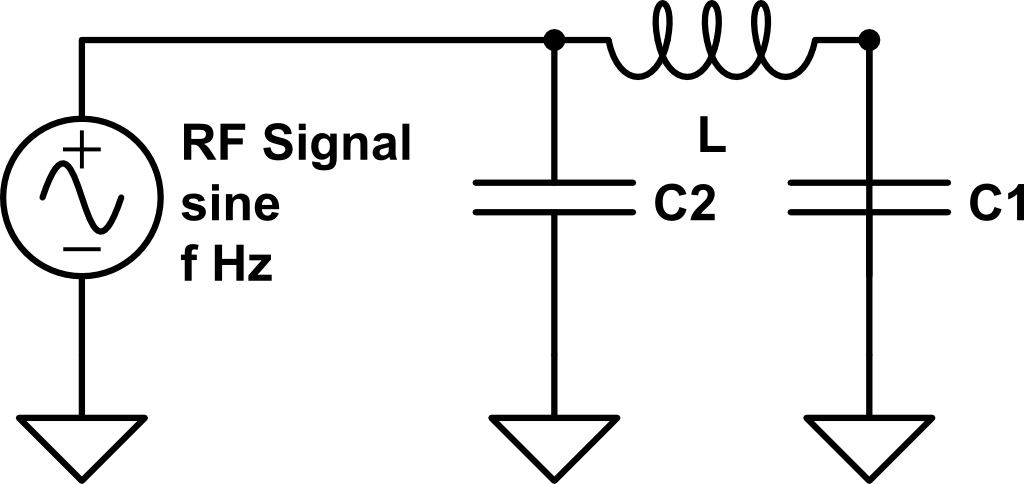
\includegraphics[width=.5\textwidth]{eom-tank-cirucuit1.png}
    \caption{EOM tank circuit board schematic (non-ideal component)}
    \label{fig:eom-tank-cirucuit1}
\end{figure}

The task of constructing an EOM at a particular modulation frequency can be be roughly broken into the following three steps:
\par
Firstly, the LC circuit is in place to act as an amplifier so that the EOM can driven with low-power RF source of $<$ 1W, yet still providing significant electric field across the crystal for phase modulation. 
\par
Since we have an intended EOM modulation frequency frequency $f_0$, and the capacitance of the EOM crystal $C_1$ is fixed, we need to measure $C_2$ in order to backcalculate the inductor $L$ needed. Since the capacitor is small at the $pF$ level, we need to characterise $C_1$ by hooking it up with a suitable resistor, sending a square wave through it and determine its response time. Although the capacitance of the crystal should be predominantly determined by the crystal dielectric, my observation showed that the way that it's glued to the tank circuit also affects. I used silver containing glue spreaded evenly under the crystal and attached the crystal to the EOM tank circuit board's exposed copper section. The conductive glue is such that bottom of the crystal has a common ground hence electric field across the crystal will be near homogeneous as wanted. For my crystal with the way that it was glued, $C_1 \approx 3 \mu F$.
%TODO: insert measurements of crystal capacitance here
\par
After measurement of $C_1$, we can estimate the capacitance of the tank circuit board to be $C' = \frac{C_1C_2}{C_1+C_2} \approx C_1$. This is because $C_1 \gg C_2$ where $C_2$ is a coupling capacitor that will be explained later. The resonant frequency of the tank circuit can be estimated to be $f = \frac{\omega}{2\pi} = \frac{1}{2\pi\sqrt{LC'^2}}$. Rearranging to get $L = \frac{1}{(2\pi f C_1)^2}$, to get a resonant frequency of about 35 MHz, a $2 \mu H$ inductor is needed, the closest off-the-shelf inductor is $2.2 \mu H$. 
\par
Secondly, the overall impedance of the EOM tank circuit needs to be matched to be $50\ohm$ such such that RF signal going to the EOM tank will be mostly absorbed and not reflected. In order tune the overall impedance of the EOM tank circuit, a coupling capacitor $C_2$ is added as shown in schematic \ref{fig:eom-tank-cirucuit1}. The overall loss of the EOM tank circuit can be modelled by a resistor $R_p$ as shown in Fig \ref{fig:eom-tank-cirucuit2}. Here we consider the components ideal. Note that parasitic resistance can be dependent on signal frequency, environment and many others. Here take it as $ R_p \approx 15 \Ohm$ based on Meng Khoon's note. However, much more careful characterisations of the circuit can be done. The coupling capacitor does not affect the tank circuit resonant frequency significantly as $C_1 \gg C_2$. so $C' = \frac{C_1C_2}{C_1+C_2} \approx C_1$ as mentioned earlier.  

\begin{figure}[H]
    \centering
    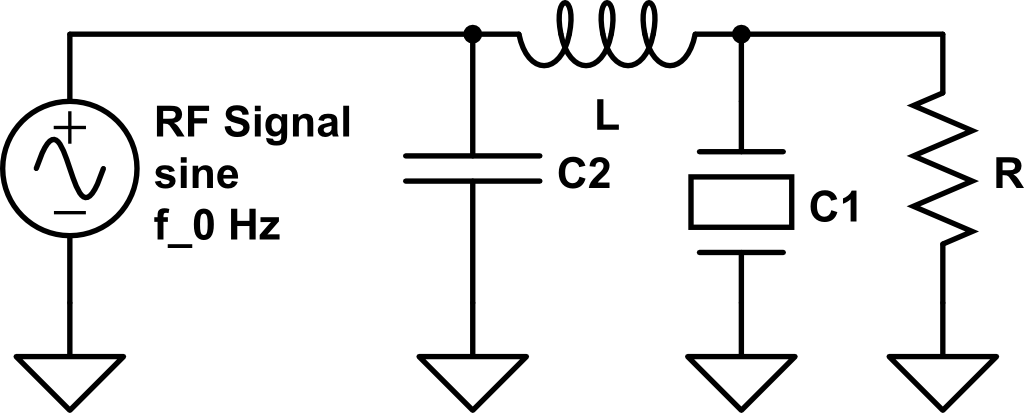
\includegraphics[width=.8\textwidth]{eom-tank-cirucuit2.png}
    \caption{EOM tank circuit, modelling overall loss}
    \label{fig:eom-tank-cirucuit2}
\end{figure}

We can calculate the overall impedance of the circuit based on this model. Setting overall impedance to be $50\Ohm$, the needed $C_2$ can be backcalculated to be $C_2 = \frac{\sqrt{50/R_p -1}}{50} \approx 93.8 nF$ which is indeed much smaller than $C_1 \approx 3 \mu F$. Choose a variable capacitor around this range of capacitance. 
\par
Lastly set up a measurement circuit as shown in Fig \ref{fig:eom-freq-measurement-setup.png}. Tune the variable capacitor until reflected signal from the EOM tank circuit board is minimum. Note that most variable capacitor has a tuning range of less than $360\degree$, so tune slowly until the valley shown on the spectrum analyser is the deepest. 

\begin{figure}[H]
    \centering
    \includegraphics[width=.8\textwidth]{EOMboard.png}
    \caption{EOM board}
    \label{fig:EOMboard}
\end{figure}

\begin{figure}[H]
    \centering
    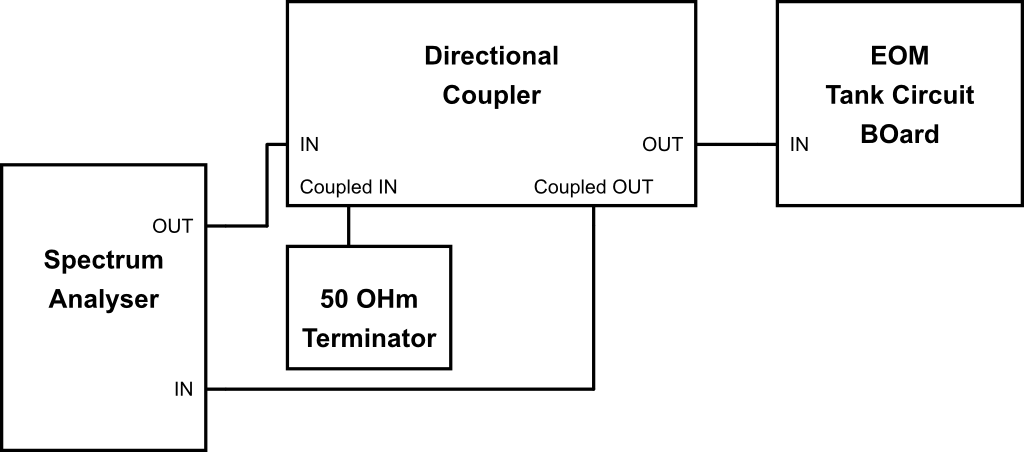
\includegraphics[width=0.8\textwidth]{eom-freq-measurement-setup.png}
    \caption{EOM frequency measurement setup}
    \label{fig:eom-freq-measurement-setup.png}
\end{figure}

After tuning the variable capacitor, my EOM tank circuit (Fig \ref{fig:EOMboard}) board has a resonant frequency $f_0 \approx 17.95 MHz$, see Fig \ref{fig:EOMfrequencyMeasurement}. 

\begin{figure}[H]
    \centering
    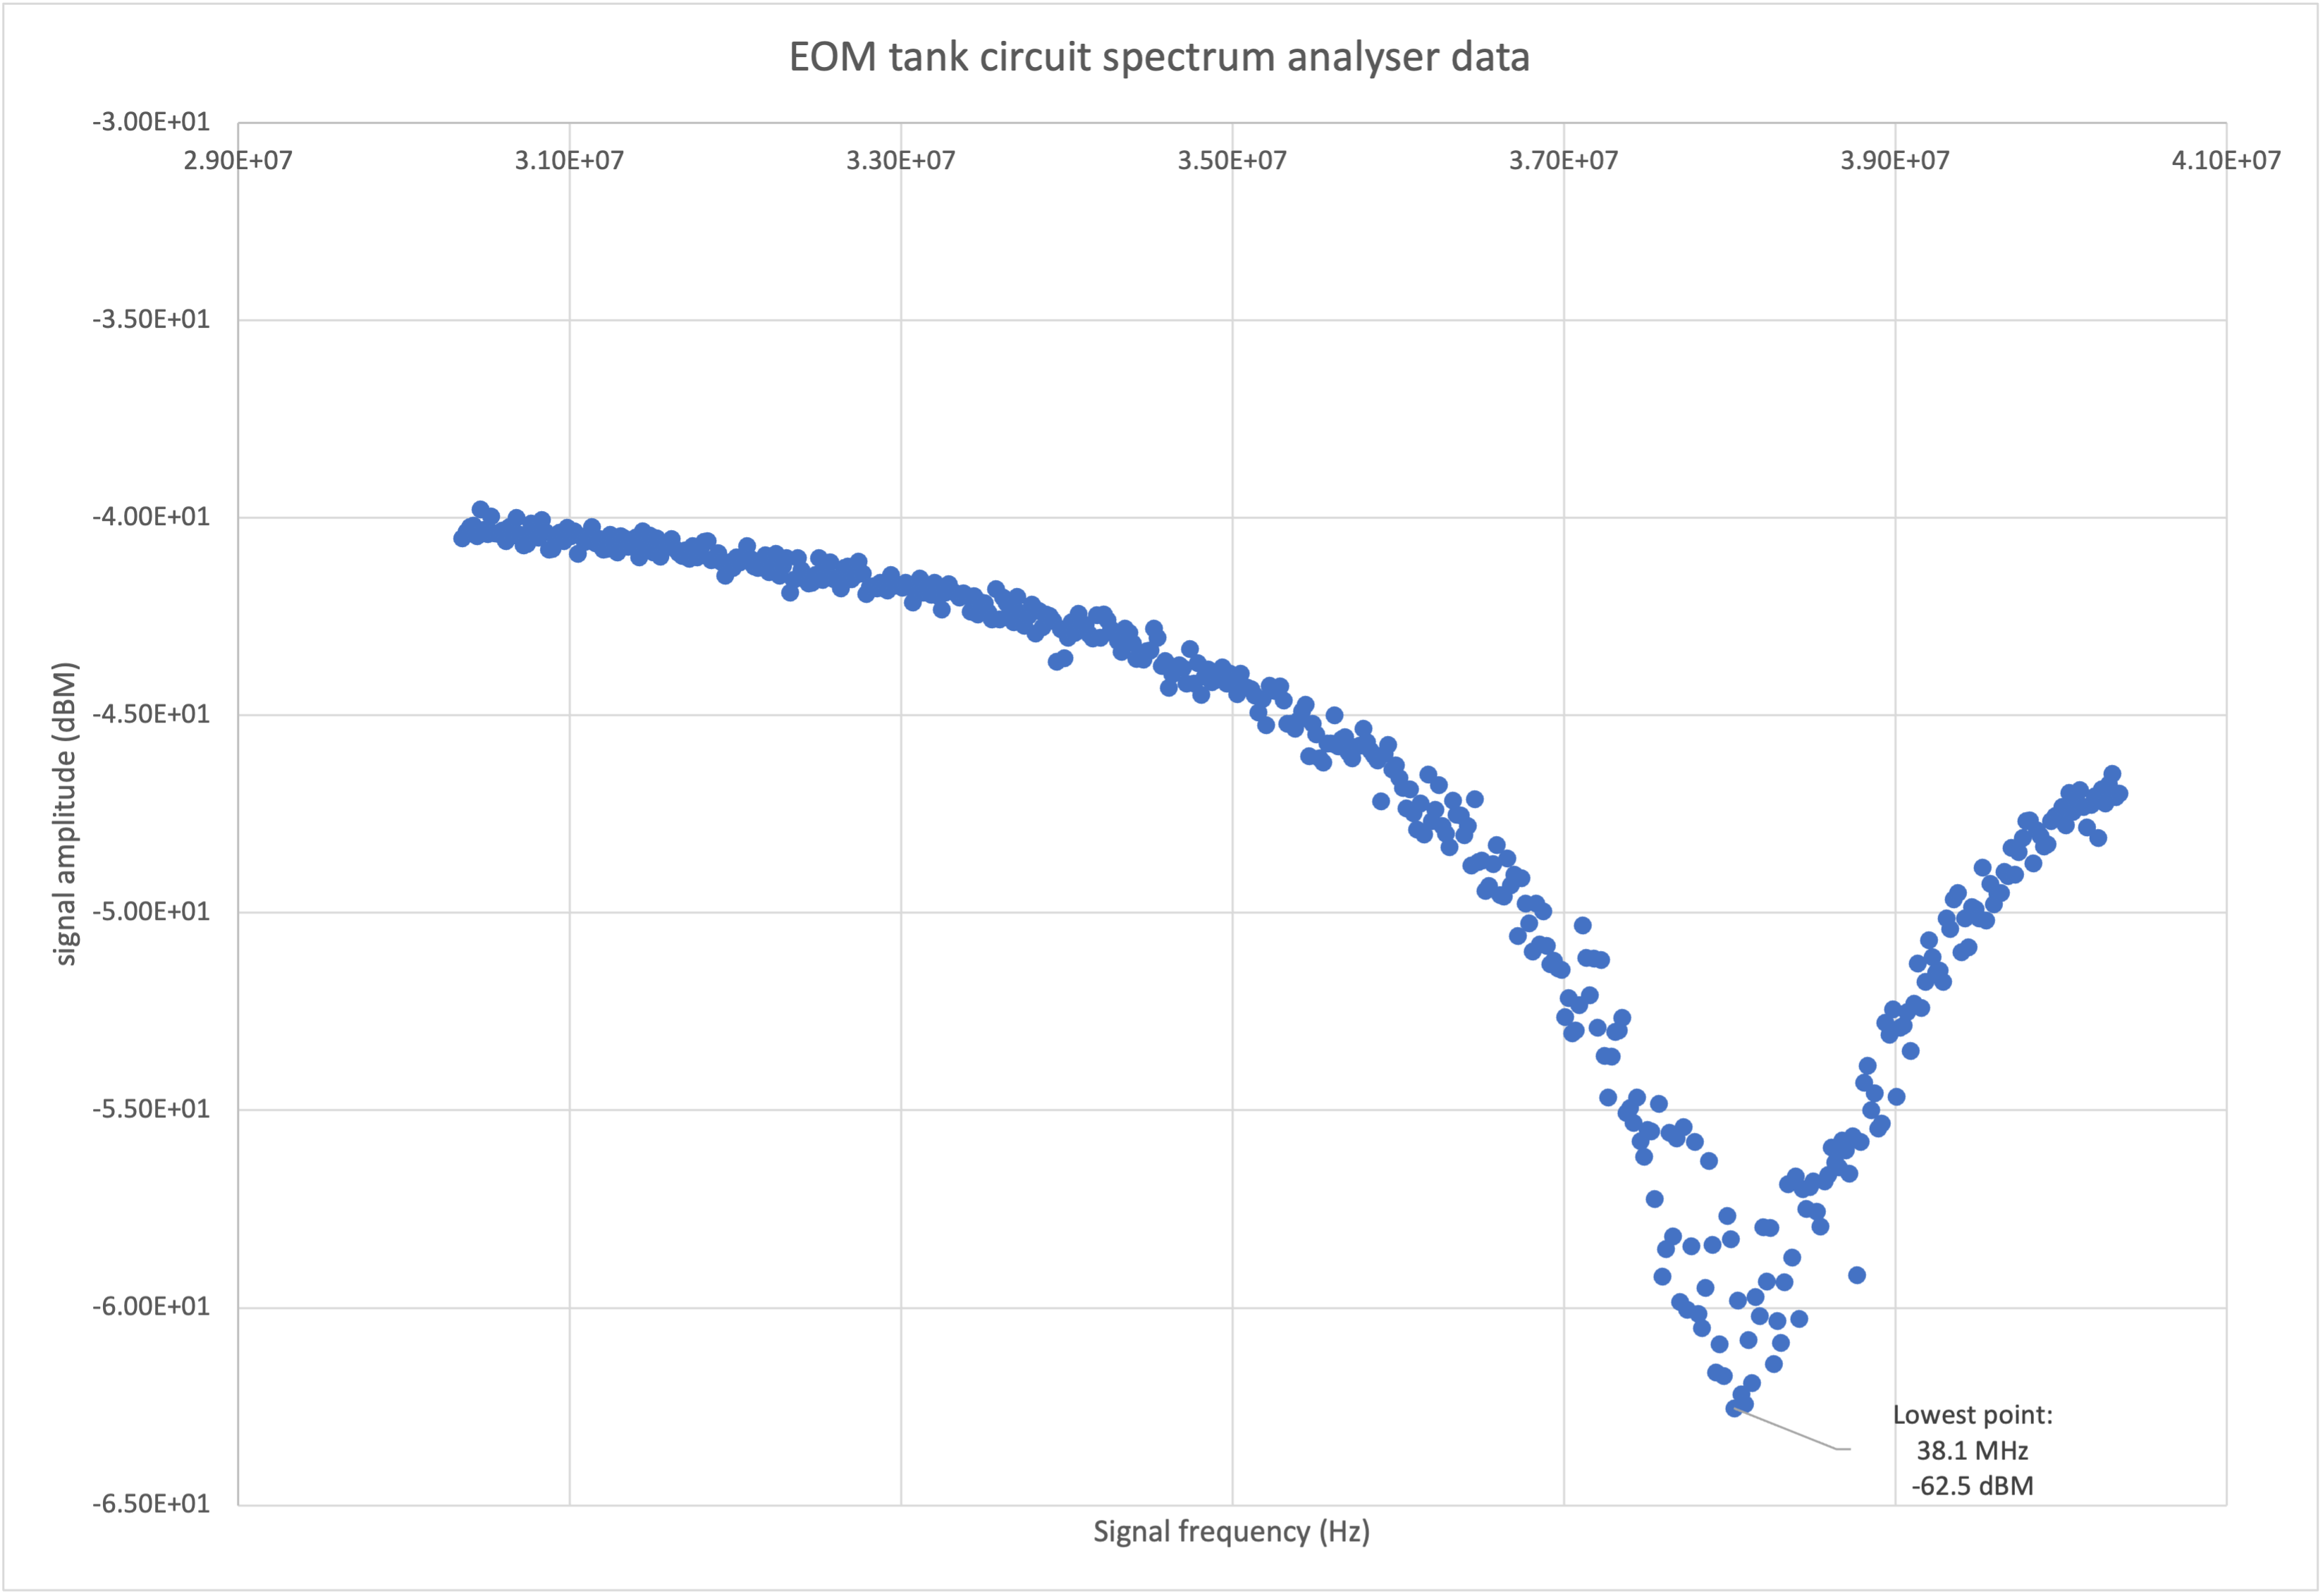
\includegraphics[width=0.8\textwidth]{EOMfrequencyMeasurement.png}
    \caption{EOM tank circuit frequency measurement setup}
    \label{fig:EOMfrequencyMeasurement}
\end{figure}

A final word on EOM construction: To improve on the Q-factor of the EOM tank circuit, parasitics of the circuit need to be better charactersied and subsequently matching impedance better. A better impedance matching will lead to higher efficiency of absorption of input RF signal. A small-voltage RF signal can bring about more significant modulation. However, my EOM as it currently is suffices for my subsequent task. 
%TODO: measure Q-factor of my EOM board
%TODO: insert an image of my actual EOM board here

\section{Fabry-Perot Cavity}
\subsection{Theory}
Laser resonators are open structures containing two or more mirrors that are aligned to produce optical feedback to the gain element. In the simplest case, a resonator consists of two aligned mirrors. These mirrors are called end mirrors and define the optical cavity. Optical radiation circulates within the cavity, bouncing back and forth between the end mirrors and passing through the gain element. An optical resonator can be characterised by the following parameters: 
\begin{enumerate}
    \item number of mirrors constituting the resonator
    \item focal length of mirrors
    \item radius of mirrors (usually small relative to cavity length)
    \item length of cavity
    \item reflectivity of mirrors
    \item other optical losses: how good is the vacuum in the cavity and so on
\end{enumerate}
What's relevant to this report is a particular type of optical resonator: confocal Fabry-Perot cavity. Fabry-Perot cavities are optical cavities with two parallel mirrors. Confocal Fabry-Perot cavities have focal points of the two concave mirrors overlapping at the center of the cavity as shown in Fig \ref{fig:confocalCavity}. The confocal cavity I used in experiment has a cavity length of L=15cm. 

\begin{figure}[H]
    \centering
    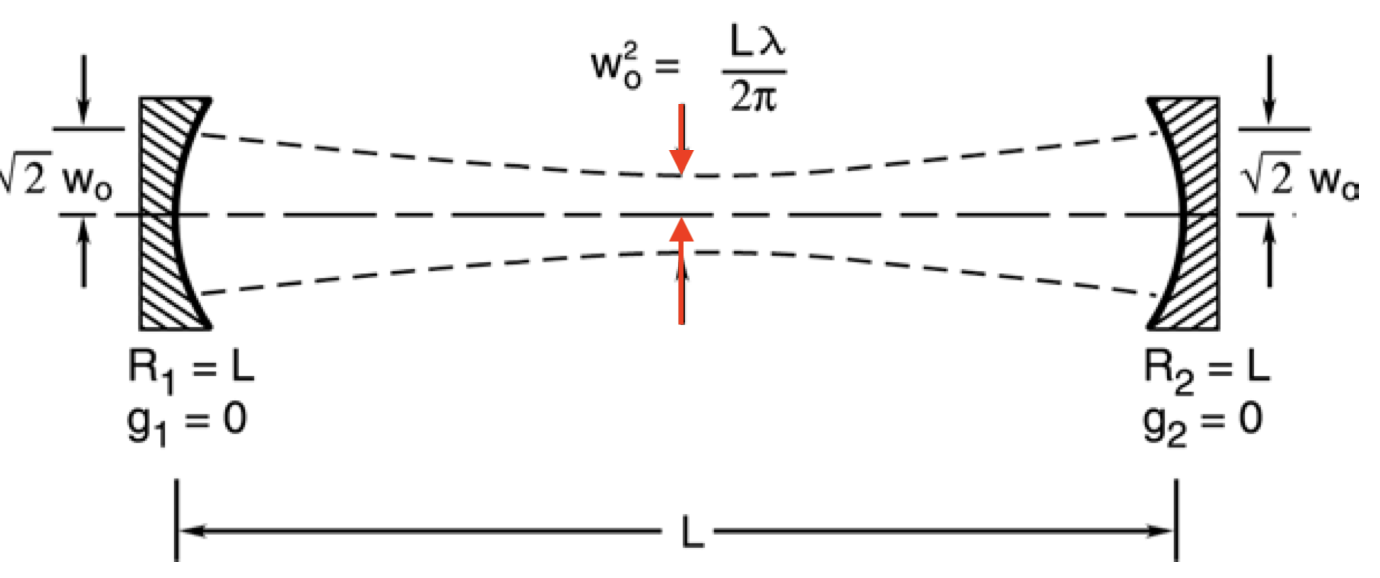
\includegraphics[width = .8\textwidth]{confocalCavity.png}
    \caption{Confocal cavity}
    \label{fig:confocalCavity}
\end{figure}

One good way to measure the frequency of a laser's beam is send it into a Fabry-Perot cavity and look at what gets transmitted (or reflected). Light can only pass through a Fabry-Perot cavity if twice the length of the cavity is equal to an integer number of wavelengths of the light. Or equivalently put, the frequency of the light's electromagnetic wave must be an integer number times the cavity's free spectral range $\Delta \nu_{fsr} \equiv c/2L$, where $L$ is the length of the cavity and $c$ is the speed of light. For my case $\Delta \nu_{fsr} \approx 1GHz$. The cavity acts as a filter, with transmission lines, or resonances, spaced evenly in frequency every free spectral range. Fig \ref{fig:cavityTransmission}  shows a plot of the fraction of light transmitted through a Fabry-Perot cavity versus the frequency of the light. \cite{PDHintro}\cite{fundamentalsOfPhotonics}

\begin{figure}[H]
    \centering
    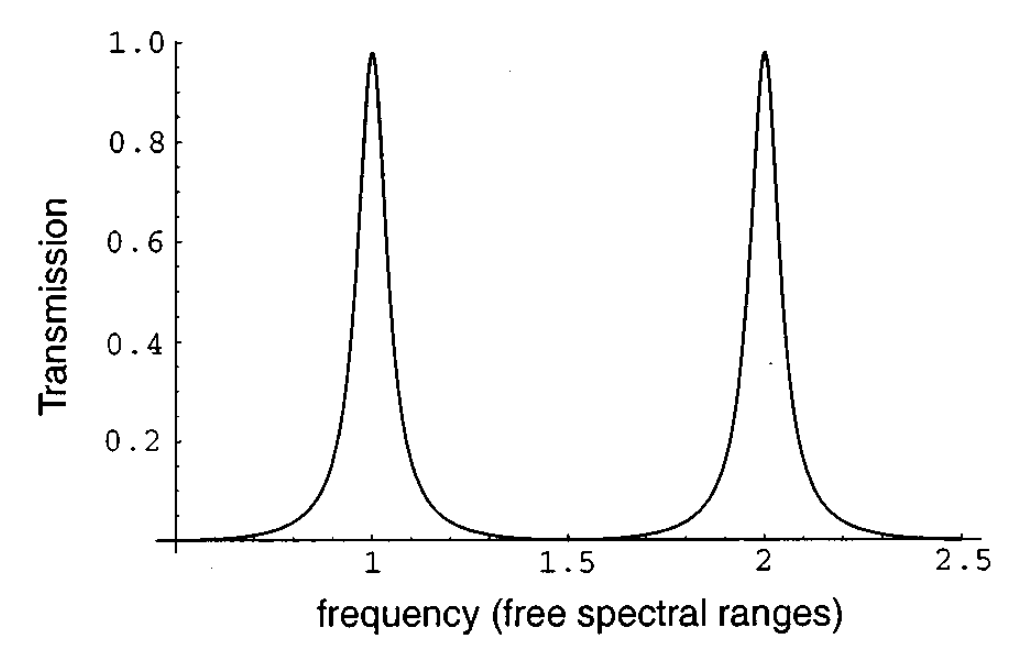
\includegraphics[width=.8\textwidth]{cavityTransmission.png}
    \caption{Cavity transmission}
    \label{fig:cavityTransmission}
\end{figure}

\subsection{Laser beam - Cavity Coupling}
To couple a well collimated laser beam with beam radius $\omega_1$ (see section on laser beam collimation and characterisation in this report) into a Fabry-Perot cavity, follow these steps: 
\begin{enumerate}
    \item Choose a thin lens (with relevant AR coating) of focal length $f$ to focus the laser beam from radius $\omega_1$ to $\omega_0$ at the center of the cavity. Gaussian beams have a propagating spherical wavefront, and each Gaussian beam is uniquely characterised by its beam waist, here being $\omega_0$. In the context of a confocal cavity, when a Gaussian has beam waist $\omega_0 = \frac{L\lambda}{2\pi}$ as shown in Fig \ref{fig:confocalCavity} the Gaussian beam spherical wavefront at the mirrors will match the curvatures of the mirrors, hence leading to stable standing waves to establish in the cavity. In my case, consider $L=15$ cm, $\lambda = 935.18848$ nm,  $\omega_0$ = $0.000149419$ m.
    
    \item To determine the focal length $f$, we consider how parameters of a Gaussian beam transforms through a thin convex lens (see \cite{principleOfLasersOrazio} for details). Approximately, we have $\omega' \approx \frac{\lambda f}{\pi \omega}$. Where, $\omega'$ is the 'image'-side beam waist, $\omega$ is the 'object'-side beam waist, $\lambda$ is laser beam wavelength, $f$ is the thin lens focal length. In my case, consider $\lambda = 935.18848$ nm, $\omega'$ = $0.000149419$ m. $\omega = 1.1$ mm (image-side beam radius is estimated to be so through beam characterisation) $f = frac{\omega' \pi \omega_1}{\lambda} \approx 0.552139m \approx 550mm$. However, using a lens of such focal length was not practical due to space constraint on the optical table, I used a $f=150mm$ thin lens as it was the longest focal length lens available off-the-shelf. 
    
    \item Pass the laser beam through at least one mirror before entering the cavity to obtain at least 2 points of adjustment. See Fig \ref{fig:laserCavityCoupling} in Appendix for a hand-written note on how to adjust the mirrors (or fibre mount) for optical coupling using a card (either normal paper or IR paper depending on wavelength) with a hole. 

    \item Lastly send a triangle wave signal of appropriate $V_{pp}$ to the piezo actuator to scan the cavity length across a certain range. The $V_{pp}$ needed depends on the scanning range needed and the behaviour of the piezo actuator. See chapter 2 of \cite{FundamentalPrinciplesofEngineeringNanometrology} for details on piezo actuators. For my case, after testing, a triangle wave generator board producing $\pm 5$V, together with a voltage gain board of coefficient 19 is used to produce a $V_{pp} \approx 190$V. See Fig \ref{fig:935cavityScan}, yellow line comes from a sync port of the triangle wave generator, green line comes from a photodiode at the exit end of cavity. Notice that "half a triangle" covers two peaks (not optimised in this image, but it was optimised after the image was taken), indicating that the cavity scan range is sufficient to cover a free spectral range of my cavity. Fine tune the cavity to obtain highest peaks possible 
    \par
    Caution: 
    \begin{enumerate}
        \item The piezo actuator might fracture under high negative voltage, so avoid sending in negative voltage to it. For my case, I used a offset gain board to make sure the triangle wave sits above 0V.
        \item The voltage sent to the piezo actuator is HV, be cautious and remember to electrically insulate the cavity from the optical table.
    \end{enumerate}
\end{enumerate}

\begin{figure}[H]
    \centering
    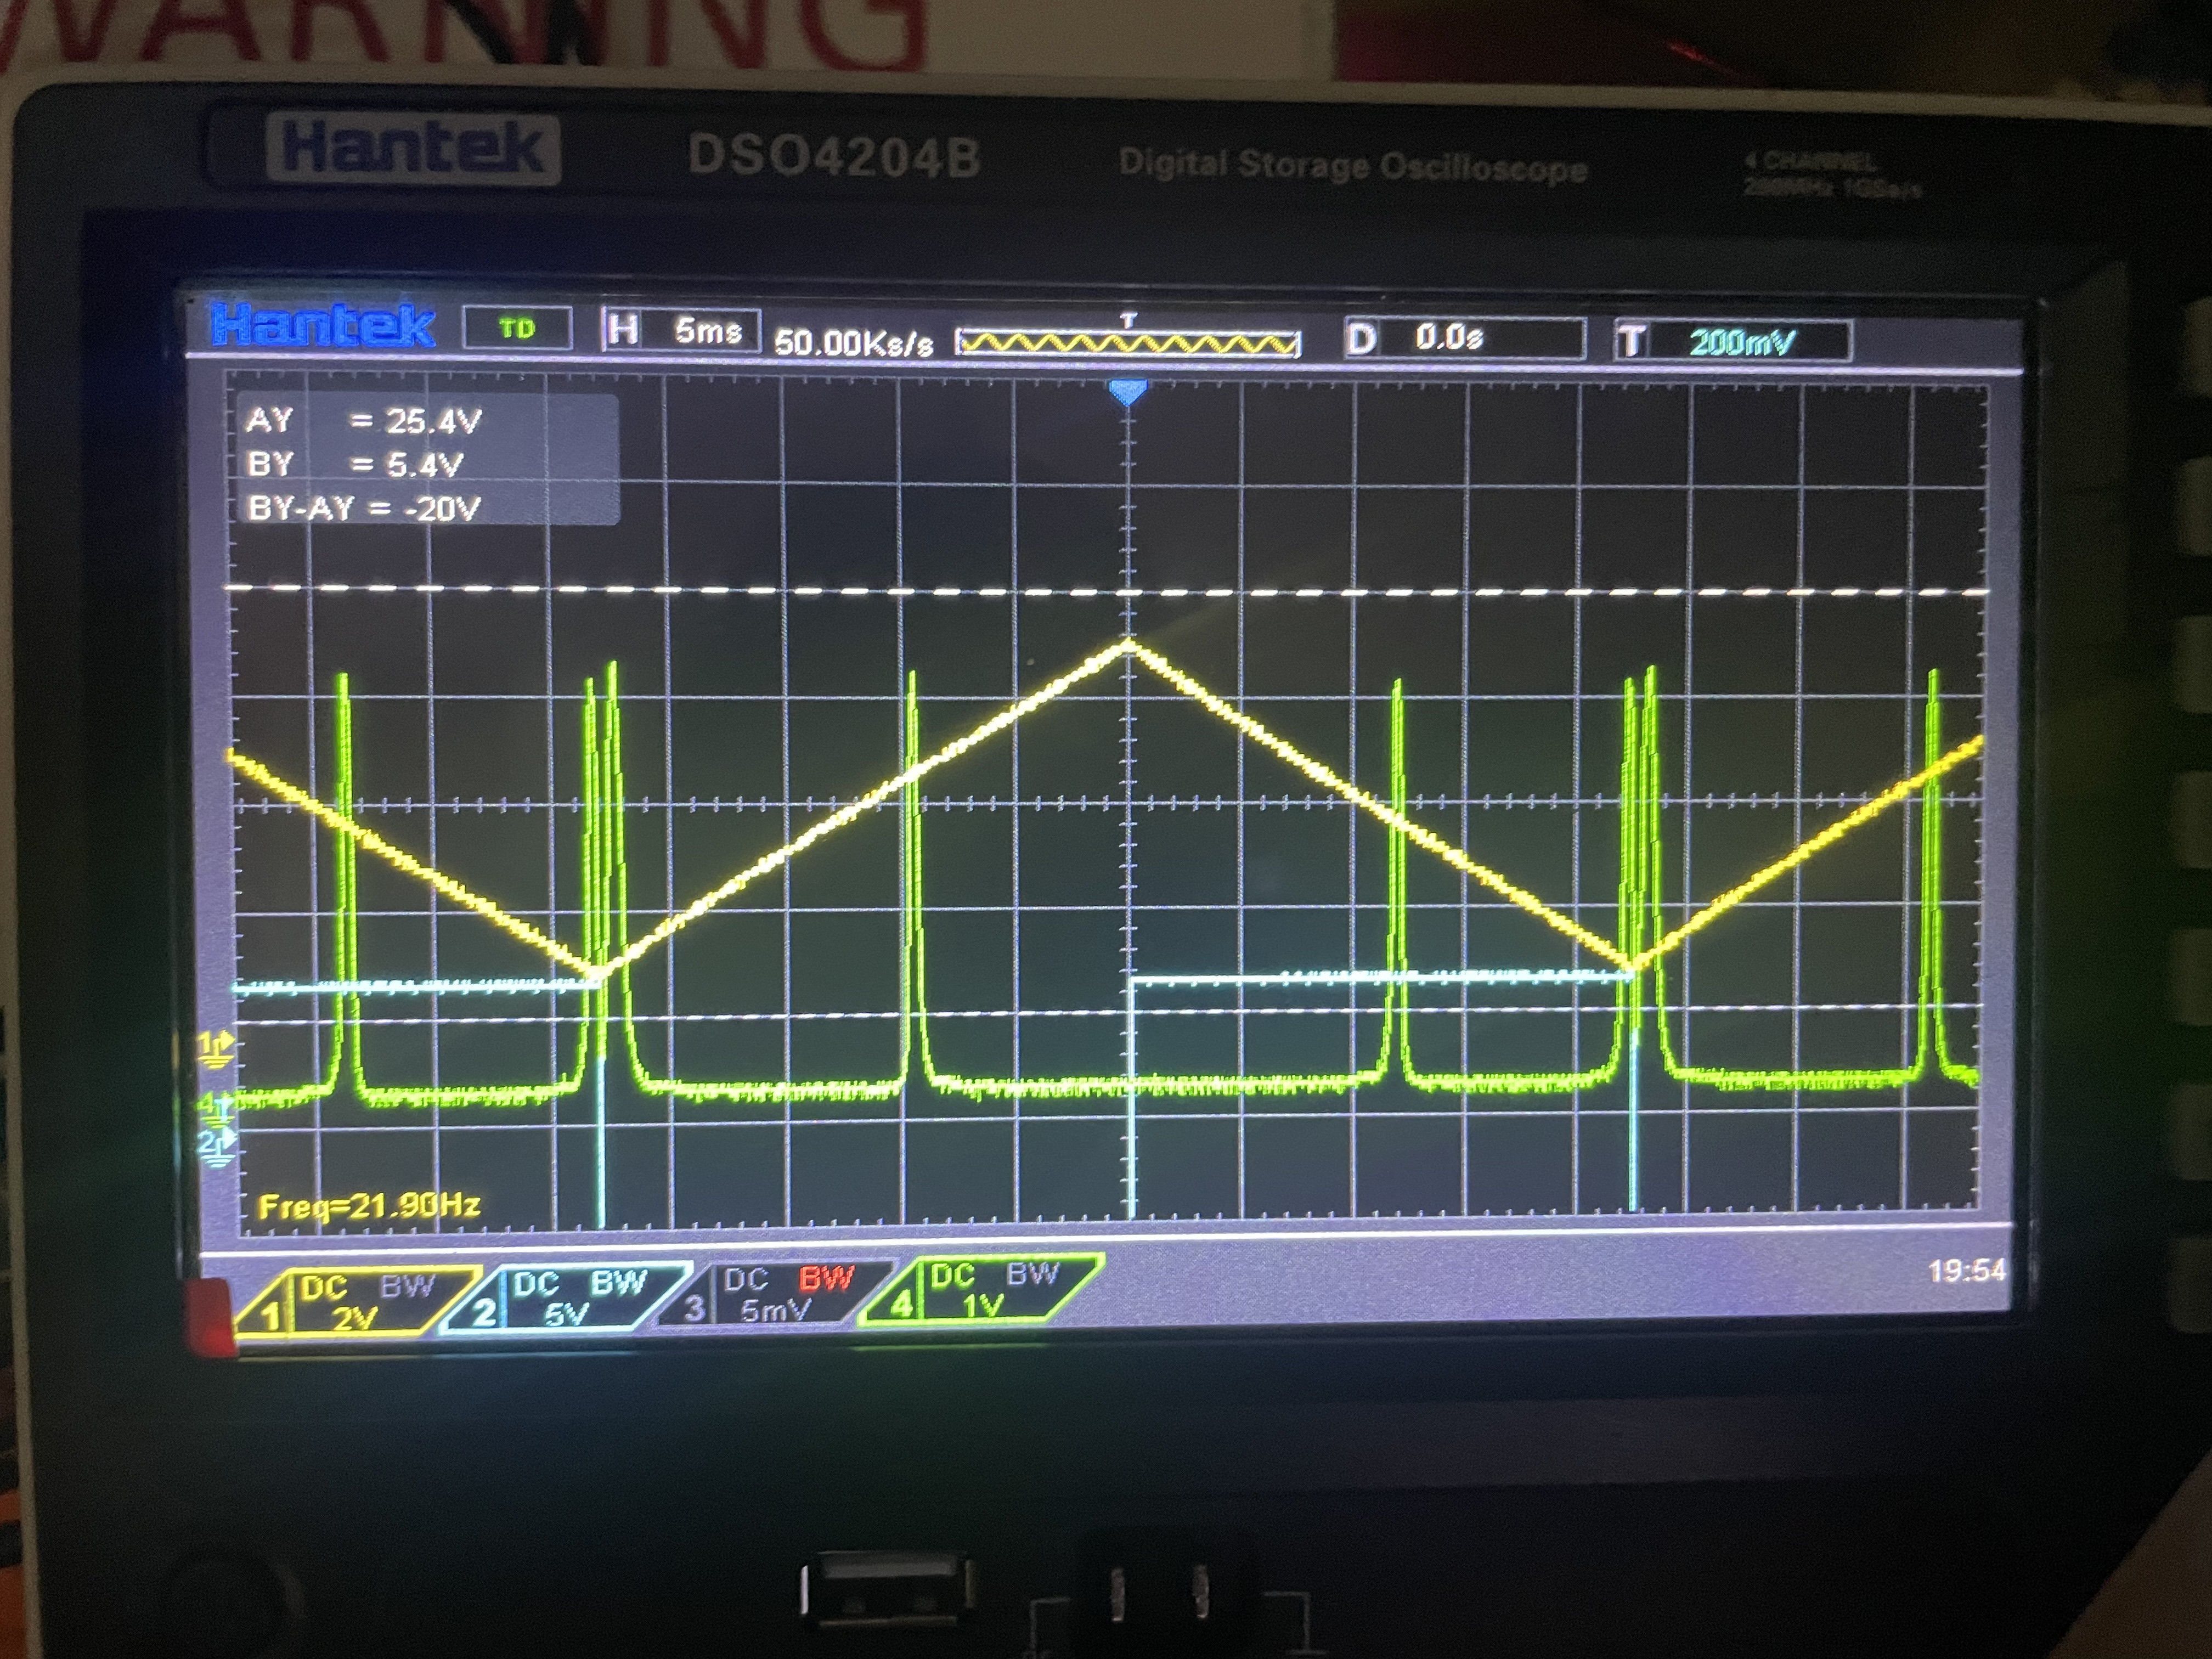
\includegraphics[width=.8\textwidth]{935cavityScan.jpeg}
    \caption{935nm laser Cavity Scan on Oscilloscope}
    \label{fig:935cavityScan}
\end{figure}

\section{PDH Cavity Lock: Actual Setup}
The actual set up of the PDH scheme is shown in Fig \ref{fig:PDHsetup}. In the red box there is the $\approx$ 738nm laser fiber output, polarisation cleanup waveplate pair and EOM crystal connected to local oscillator. In the blue box there is $\approx$ 935nm laser fiber output and polarisation cleanup waveplate pair. In the center row there is a beam splitter that overlaps the optical path of both 738nm and 935nm laser beams, an optical isolator formed by a PBS and a QWP for 738nm laser beam, a plano-convex lens for laser-cavity coupling, a F-P cavity connected to a triangle wave generator, lastly a detector pedal that measures transmitted intensity through the cavity. In the yellow box, a plano-convex lens focuses reflected beam from the cavity that is channelled out from the optical isolator to a fast photodiode (a transimpedance amplifier) which is then connected to a amplifier and to the mixer as shown in Fig \ref{fig:PDHlayout}. 

\begin{figure}[H]
    \centering
    \includegraphics[width=.8\textwidth]{PDHsetup.png}
    \caption{PDH Setup}
    \label{fig:PDHsetup}
\end{figure}

The electronic parts are shown in Fig ... The signal from local oscillator is split by a fifty-fifty power splitter. One branch goes to the mixer L port. The other branch goes to an amplifier before being sent to the EOM board. One thing worth noting is that when local oscillator $V_pp$ goes above 200mV, the EOM board in Fig \ref{fig:EOMboard} radiates significant RF signal such that the wavemeter located on the top rack gets affected. Fast diode signal from Fig \ref{fig:PDHsetup} yellow box connects to mixer I port. mixer R port after passing through a low-pass filter outputs the error signal shown in Fig \ref{fig:errorSignal}, where the blue curve is the error signal and the yellow curve is the transmission intensity.  Note that from the local oscillator to the I and L ports of the mixer, signals go through different lengths. Hence, the two signals need to be phase-matched in order for the error signal to be generated properly. This was done by varying the length of the BNC cable connecting the power splitter 

\begin{figure}
    \centering
    \includegraphics{}
    \caption{Caption}
    \label{fig:my_label}
\end{figure}

\begin{figure}[H]
    \centering
    \includegraphics[width=.8\textwidth]{errorSignal.png}
    \caption{Error signal}
    \label{fig:errorSignal}
\end{figure}

The error signal is sent to the PID board which then outputs a feedback signal to the "mod in" port of the triangle generator to lock the cavity length to the 738nm master laser. To show that the cavity is indeed locked, turn on the triangle wave generator scan after the lock is on. Fig \ref{fig:cavityLock1} shows that the cavity length stays locked when the triangle wave generator scans with low amplitude. Red curve is the sync signal from triangle wave generator. Yellow curve is the transmission signal. Blue curve is the error signal. Green signal is the PID output signal. It can be seen that as the triangle wave generator scans with a triangle wave, the PID feedbacks a reverse triangle wave to maintain the cavity length such that the transmission intensity (yellow curve) stays around the maximum intensity. However, the lock is not a very good one as it can be seen that the error signal (blue curve) doesn't stay close to 0 most of the time. Furthermore, as it can be seen from Fig \ref{fig:cavityLock2} and \ref{fig:cavityLock3}, as the triangle wave generator scans with greater amplitude, transmission intensity strays away from maximum intensity, indicating the lock has been broken. 

\begin{figure}[H]
    \centering
    \includegraphics[width=.8\textwidth]{cavityLock1.png}
    \caption{Cavity lock with triangle wave generator scanning at low amplitude}
    \label{fig:cavityLock1}
\end{figure}

\begin{figure}[H]
    \centering
    \includegraphics[width=.8\textwidth]{cavityLock2.png}
    \caption{Cavity lock with triangle wave generator scanning at medium amplitude}
    \label{fig:cavityLock2}
\end{figure}

\begin{figure}[H]
    \centering
    \includegraphics[width=.8\textwidth]{cavityLock3.png}
    \caption{Cavity lock with triangle wave generator scanning at high amplitude}
    \label{fig:cavityLock3}
\end{figure}

There are two major remaining tasks. Firstly, a phase delay board is needed to better matched the two signals going into the mixer to generator a better error signal. Secondly, the PID parameters need to be better tuned to tighten the feedback lock. 

\section{Possible Uses Of The Locked Cavity}
Assuming that cavity length has now been locked to the 738nm master laser. Here are a list of uses and fun projects involving the locked cavity" 
\begin{enumerate}
    \item Adding a dichoric lens and a second fast diode creates a second PHD setup for $\approx$935nm laser that can be used to frequency locking. As discussed earlier, the frequency of the $\approx$935nm laser needs to be stabilised for continuous optical repumping.
    \item As the cavity length is now stabilised, if both the 935nm and 738nm lasers' output intensity are sufficiently stable, variation in transmission intensity can be attributed to factors such as watervapor absorption of 935nm laser since this wavelength happens to be quite close to a water molecule absorption peak. 
\end{enumerate}

However, as at the moment the 738nm master laser is not properly locked to the Ytterbium atomic cell these ideas have not been executed.

\section{Conclusion}
To conclude, during my year in the laboratory I picked up various optical laboratory skills, repaired and tuned a diode laser and built a cavity lock using PDH scheme. Possible future works include optimising and characterising the cavity lock, and testing the suggested applications of the cavity lock. 

\section{Appendix}
\subsection{Gaussian Beam - Single Mode Fibre Coupling Procedure} \label{appendix:laerFibreCoupling}
\begin{enumerate}
    \item Make sure that the laser beam at least go through one mirror before being sent to the fibre mount to allow for two points of freedom. Rough align the collimated beam through the fiber mount without the fibre on. Try to center the beam through the fibre mount entry. 
    \item Screw optical fiber onto the fiber mount and attach a fiber testing pen to the exit end of the fibre. Place a piece of paper on the optical path and try to align the two spots from the diode laser and the fibre pen by iteratively adjusting the mirror and the fiber mount. 
    \item Detach the fibre pen and sent the light from the exit end of the fibre (if no light at all, go back to previous step) to a power meter and perform "Walking-the-beam" technique \cite{WalkingTheBeamThorlabs} to optimise coupling. 
    \item If the previous step doesn't go to efficiency above 50\%, turn the fiber mount lens position to optimise. Note that this is very sensitive, so adjust the fibre mount lens with small turns of about 2-3$\degree$ at a time. As the optimised position is approached, even finer adjustment is required. 
    \item Note that coupling efficiency above 60\% requires significantly more effort than described. More sophisticated techniques need to be employed. However, this methods should lead to a minimum of 60\% coupling, if not achievable consider: 
    \begin{enumerate}
        \item Clean the optics: fibre cross section and mirrors.
        \item Check whether the fibre has any leakage by using a fibre pen and look for light leakage in a dark room. 
        \item Consider tuning in a larger range to get out of a possible local maximum. 
    \end{enumerate}
\end{enumerate}
\begin{figure}[H]
    \centering
    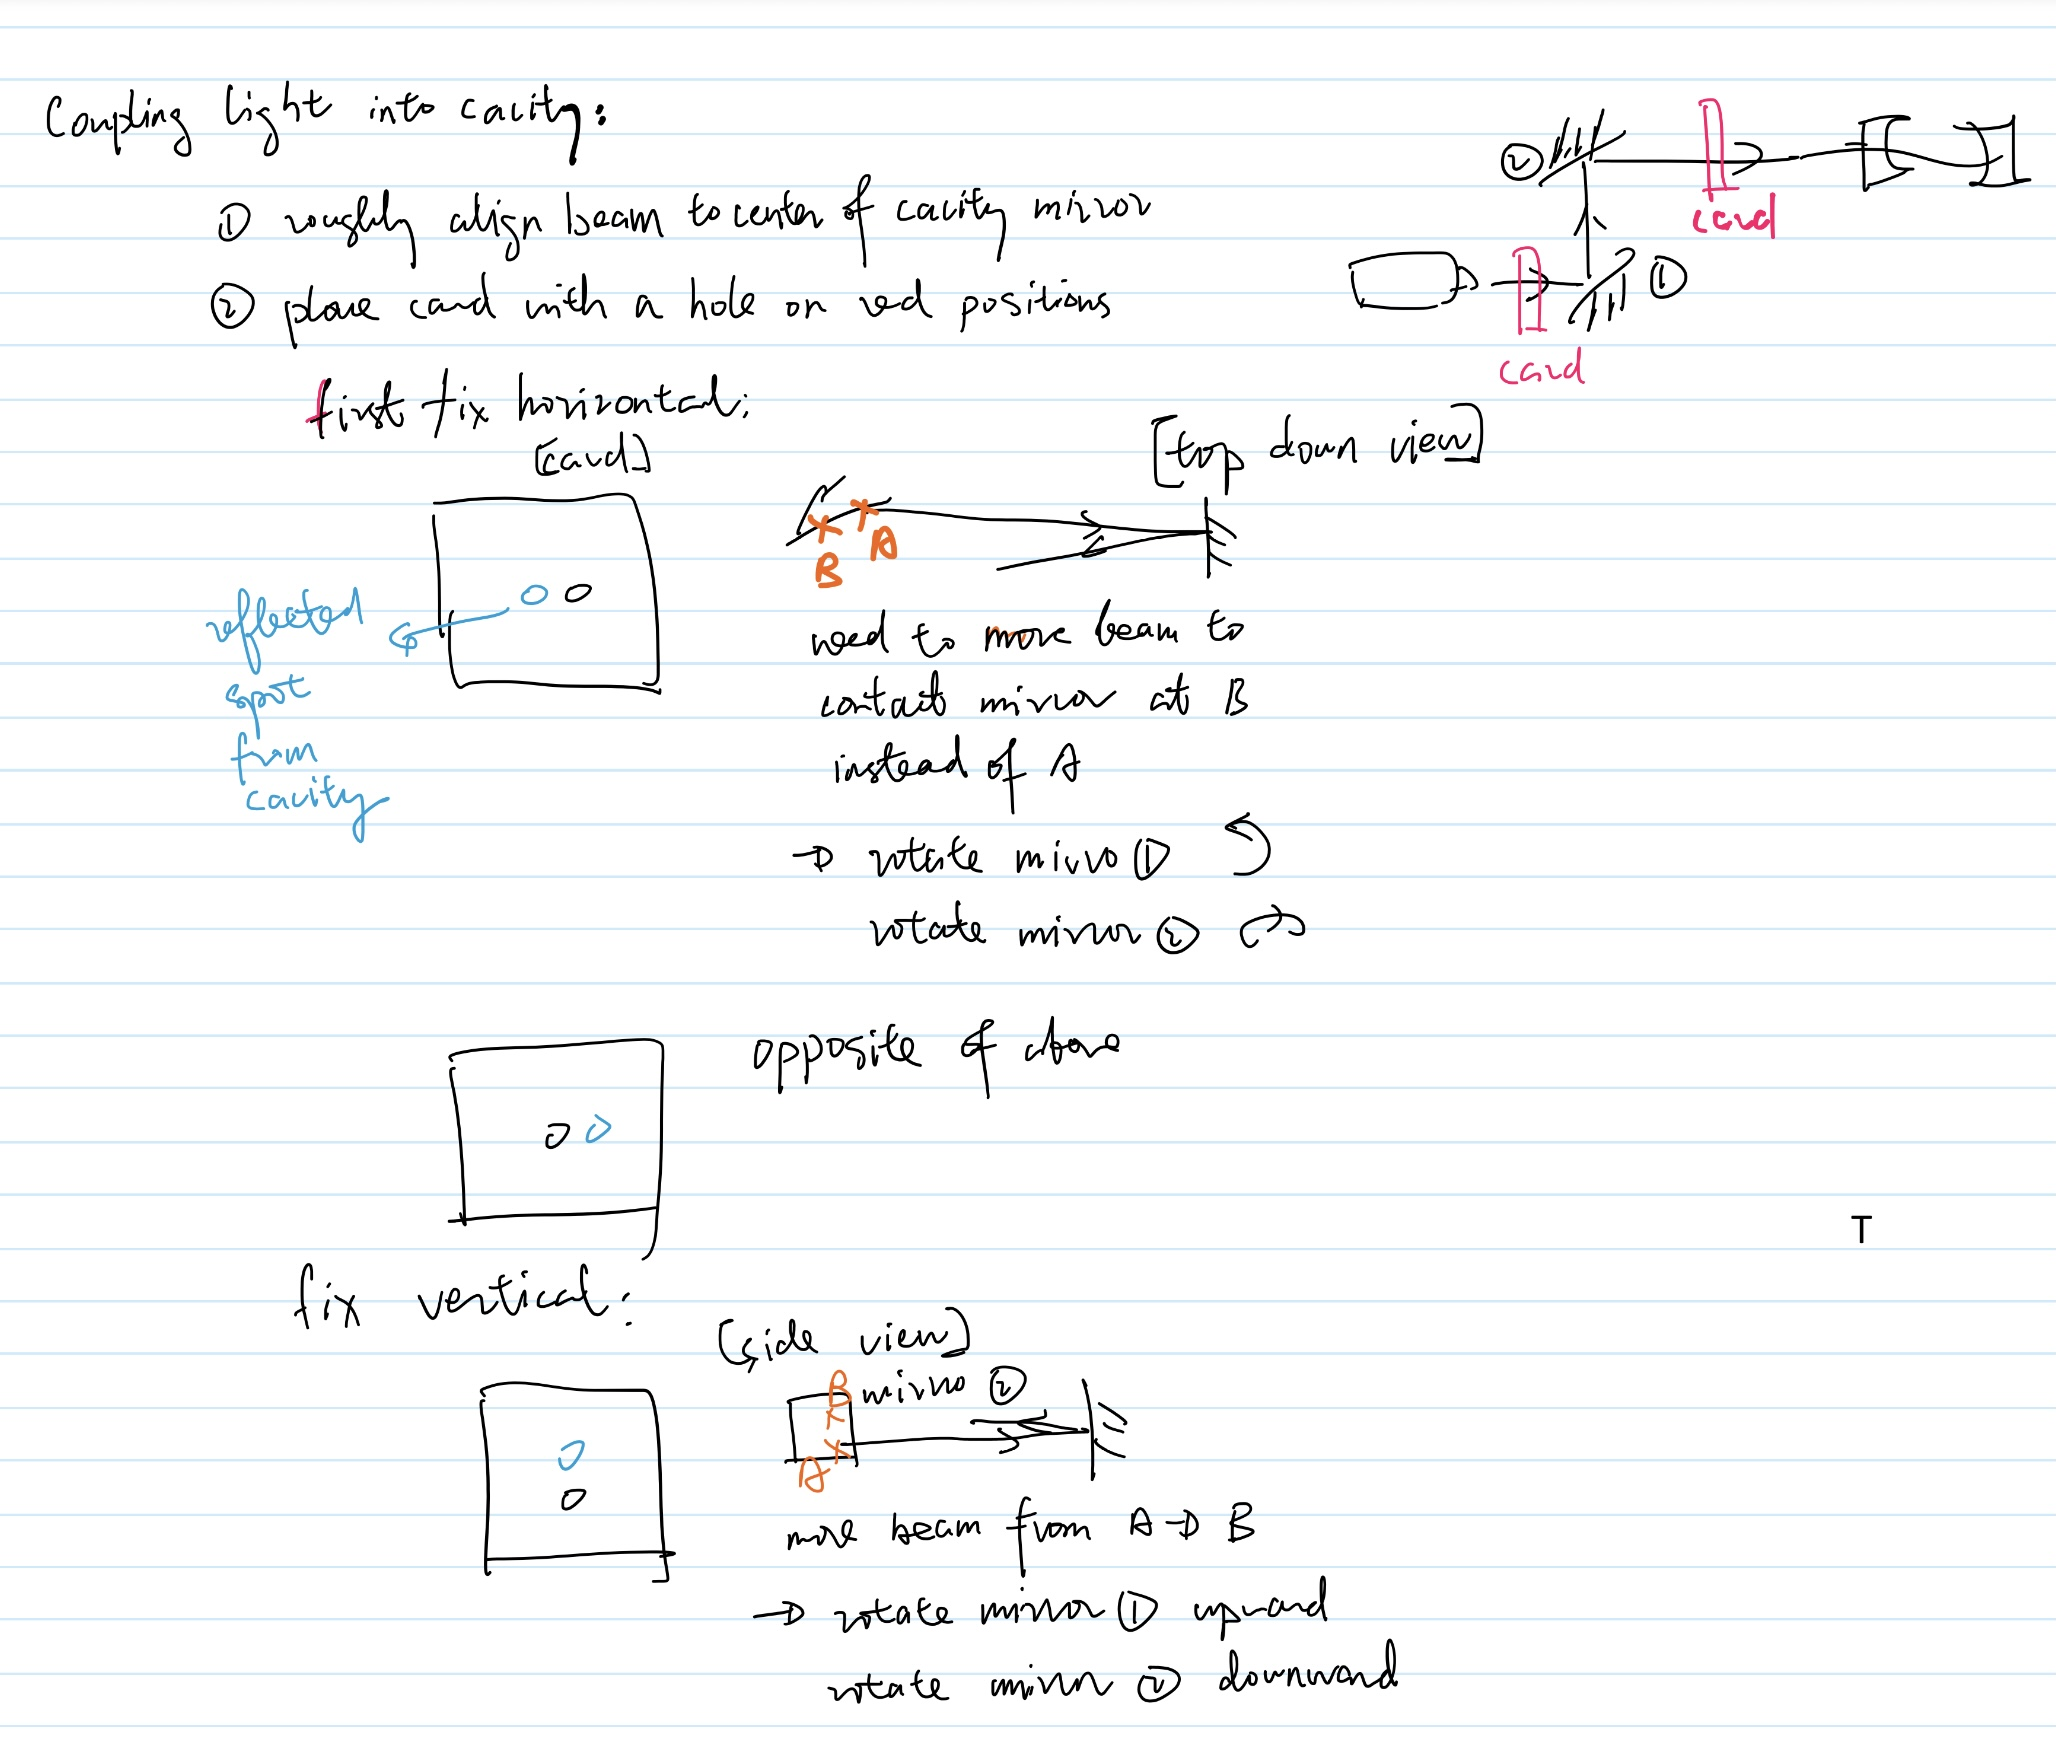
\includegraphics[width=\textwidth]{laserCavityCoupling.jpg}
    \caption{Laser beam - Cavity Coupling Note}
    \label{fig:laserCavityCoupling}
\end{figure}

\lstinputlisting[language=Python, linewidth=0.9\textwidth, basicstyle=\small\ttfamily, breaklines=true, breakatwhitespace=true, caption = Gaussian Beam Characterisation code with a CCD camera, label=code:gaussianBeamCharacterisation]{gaussianBeamCharacterisation.py}

\lstinputlisting[language=Python, linewidth=0.9\textwidth, basicstyle=\small\ttfamily, breaklines=true, breakatwhitespace=true, caption=Knife Edge Measurement Data Collection, label=code:knifeEdgeMeasurementDataCollection]{knifeEdgeMeasurementDataCollection.py}

\lstinputlisting[language=Python, linewidth=0.9\textwidth, basicstyle=\small\ttfamily, breaklines=true, breakatwhitespace=true, caption=Knife Edge Measurement Data Processing, label=code:knifeEdgeMeasurementDataProcessing]{knifeEdgeMeasurementDataProcessing.py}


\bibliographystyle{plain}
\bibliography{bibliography.bib}

\end{document}
